\documentclass[10pt,a4papper]{article}
\usepackage{graphicx}
\usepackage{amsmath}
\usepackage{amssymb}
\usepackage{cancel}
\usepackage{multicol}
\usepackage{blindtext}
\usepackage{tikz,pgfplots}
\usepackage[hidelinks]{hyperref}
\usepackage[left=2.00cm, right=3.00cm, top=2.00cm, bottom=2.00cm]{geometry}
\usetikzlibrary{arrows,scopes}
\usetikzlibrary{angles,quotes}
\usetikzlibrary{snakes,shapes}
\usetikzlibrary{decorations.pathreplacing}
\usetikzlibrary{calc}
\tikzset{>=latex}
\setlength{\parindent}{0cm}
\author{Angel Fdo. García Núñez}
\date{Enero 18, 2023}
\title{Estadisitica}

\begin{document}

\Huge
Pozo cuadrado infinito\\

Angel Fernando García Núñez


\Large
\newpage
\[\text{Potencial}\]

\[V(x)=
\left\{\begin{array}{lll}
0 & : & x\in(0,a)\\
\infty & : & x\not\in(0,a)
\end{array}\]

\begin{center}
  \begin{tikzpicture}
    \coordinate (O) at (0,0);
    \coordinate (x) at (5,0);
    \coordinate (V) at (0,5);
    \coordinate (o) at (0,-0.2);
    \coordinate (op) at (0,4);
    \coordinate (a) at (4,-0.2);
    \coordinate (ap) at (4,4);

    \draw[->](-1,0)--(x) node[right]{$x$};
    \draw[->](0,-0.2)--(V) node[above]{$V(x)$};
    \draw[line width=1pt,->](a) node[below]{$a$}--(ap);
    \draw[line width=1pt,->](o) node[below=2, right]{$0$}--(op);
  \end{tikzpicture}
\end{center}

\[\textbf{Ecuación de Schrödinger Independiente del tiempo}\]

\[\hat H\psi=E\psi\quad\to\quad
-\frac{\hbar^2}{2m}\frac{d^2\psi}{dx^2}+V(x)\psi(x)=E\psi(x)\]

\newpage
\[\text{Regiones I $(x\leq 0)$ y III $(x\geq a)$}:\]

\[V(x)=\infty\]

\[\text{Función de onda que soluciona la ecuación de Schrödinger}\]

\[\psi_I(x)=\psi_{III}(x)=0\]

\[-\frac{\hbar^2}{2m}\frac{d^2\psi_I}{dx^2}+V(x)\psi_I(x)=E\psi_I(x)\quad\to\quad
-\frac{\hbar^2}{2m}\frac{d^2(0)}{dx^2}+V(x)(0)(x)=E(0)(x)\]

\[\boxed{0=0}\]

\[-\frac{\hbar^2}{2m}\frac{d^2\psi_{III}}{dx^2}+V(x)\psi_{III}(x)=E\psi_{III}(x)\quad\to\quad
-\frac{\hbar^2}{2m}\frac{d^2(0)}{dx^2}+V(x)(0)(x)=E(0)(x)\]

\[\boxed{0=0}\]

\newpage
\[\text{Región II $(x\in(0,a))$}:\]

\[V(x)=0\]

\[-\frac{\hbar^2}{2m}\frac{d^2\psi_{II}}{dx^2}=E\psi_{II}(x)\]

\[\frac{d^2\psi_{II}}{dx^2}+k^2\psi_{II}(x)=0\quad:\quad k^2=\frac{2mE}{\hbar^2}\]\\

\[\text{Solución:}\]

\[\psi_{II}(x)=A\cos kx+B\sin kx\]\\

\[\text{Condiciones de frontera por continuidad}\]

\[\psi_I(0)=\psi_{II}(0)\quad,\quad\psi_{II}(a)=\psi_{III}(a)\quad\to\quad
\psi_{II}(0)=\psi_{II}(a)=0\]\\

\[\psi_{II}(0)=A\cos k(0)+B\sin k(0)=0\quad\to\quad A(1)+B(0)=0\quad\to\quad A=0\]

\[\therefore\quad\psi_{II}(x)=B\sin kx\]

\[\psi_{II}(a)=B\sin k(a)=0\quad\to\quad B\sin ka=0\]

\[B\not=0\quad\to\quad\sin ka=0\quad\to\quad ka=n\pi\]

\[\boxed{\therefore\quad k_n=\frac{n\pi}{a}}\]

\newpage
\[\text{Energía}\]

\[\quad k_n^2=\frac{n^2\pi^2}{a^2}=\frac{2mE_n}{\hbar^2}\quad\to\quad
\boxed{E_n=\frac{n^2\pi^2\hbar^2}{2ma^2}}\]\\

\[\text{Normalización}\]

\[\int_{-\infty}^\infty|\psi(x)|^2dx=1\]\\

\[\int_{-\infty}^\infty|\psi(x)|^2dx=
B^2\int_0^a\sin^2k_nxdx=1\]\\

\[\cos(a+b)=\cos a\cos b-\sin a\sin b\]

\[\cos 2x=\cos^2x-\sin^2x=(1-\sin^2x)-\sin^2x=1-2\sin^2x\]

\[\sin^2x=\frac{1}{2}-\frac{1}{2}\cos 2x\]\\

\[\therefore\quad
\int_{-\infty}^\infty|\psi(x)|^2dx=
B^2\int_0^a\left(\frac{1}{2}-\frac{1}{2}\cos 2k_nx\right)dx=1\]

\[B^2\int_0^a\left(\frac{1}{2}-\frac{1}{2}\cos 2k_nx\right)dx=
B^2\left(\frac{1}{2}a-\frac{1}{2}\int_0^a\cos 2k_nxdx\right)=1\]

\[B^2\left(\frac{1}{2}a+\frac{1}{4}\left|\sin 2k_nx\right|_0^a\right)=
B^2\left(\frac{1}{2}a+\frac{1}{4}\sin 2k_na\right)=
B^2\left(\frac{1}{2}a+\frac{1}{4}\cancelto{0}{\sin 2n}\pi\right)=1\]

\[\frac{1}{2}aB^2=1\quad\to\quad\boxed{B=\sqrt{\frac{2}{a}}}\]

\newpage
\[\text{Función de onda y energía del sistema}\]

\[\psi_n(x)=
\left\{\begin{array}{lll}
\sqrt{\frac{2}{a}}\sin\frac{n\pi}{a}x & : & x\in(0,a)\\
0 & : & x\not\in(0,a)
\end{array}\quad,\quad
E_n=\frac{n^2\pi^2\hbar^2}{2ma^2}\]\\\\

\begin{center}
  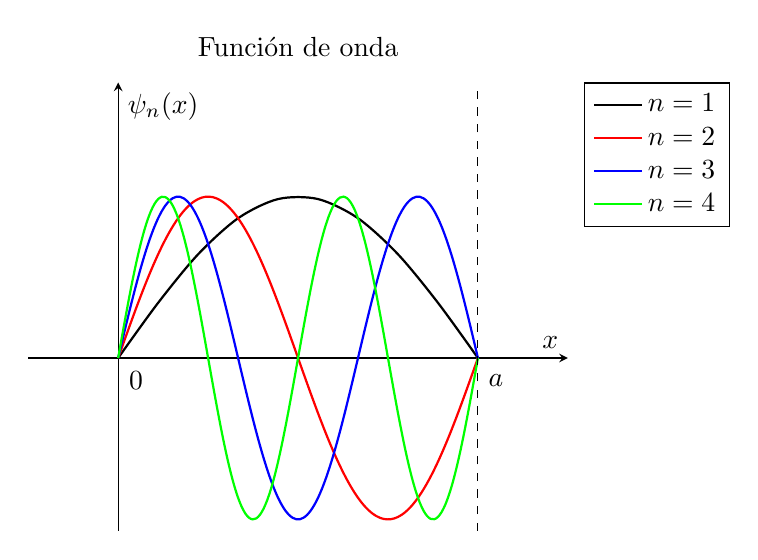
\begin{tikzpicture}
    \def\pi{3.14159}
    \def\a{4}
    \def\B{sqrt(2/\a)}
    \begin{axis}[
        title={Función de onda},
        xmin = -1, xmax = \a+1,
        ymin = -\B-0.05, ymax = \B+0.5,
        legend pos=outer north east,
        %axis lines = left,
        %hide axis,
        axis x line =center,
        axis y line =center,
        xlabel=$x$,
        ylabel={$\psi_n(x)$},
        xtick=\empty, ytick=\empty,
        legend entries={$n=1$,$n=2$,$n=3$,$n=4$}
      ]
      \addplot[smooth, thick, domain=0:\a, samples=10] {\B*sin(\pi*\x/\a r)};
      \addplot[color=red, smooth, thick, domain=0:\a, samples=100] {\B*sin(2*\pi*\x/\a r)};
      \addplot[color=blue, smooth, thick, domain=0:\a, samples=100] {\B*sin(3*\pi*\x/\a r)};
      \addplot[color=green, smooth, thick, domain=0:\a, samples=100] {\B*sin(4*\pi*\x/\a r)};
      \addplot [dashed] coordinates {(\a,-\B-0.05) (\a,\B+0.5)};
      \node at (axis cs:0.2,-0.1) {$0$};
      \node at (axis cs:\a+0.2,-0.1) {$a$};

    \end{axis}
  \end{tikzpicture}
\end{center}.\\

\begin{center}
  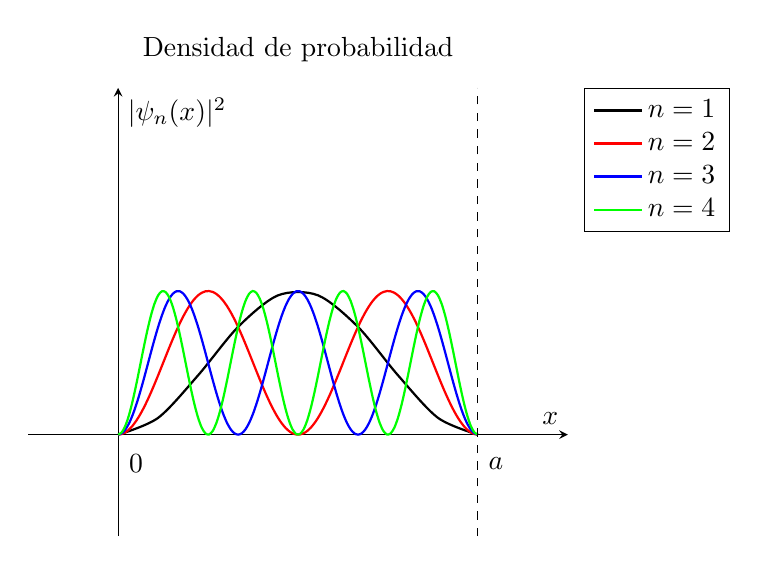
\begin{tikzpicture}
    \def\pi{3.14159}
    \def\a{4}
    \def\B{sqrt(2/\a)}
    \begin{axis}[
        title={Densidad de probabilidad},
        xmin = -1, xmax = \a+1,
        ymin = -0.5*\B, ymax = \B+0.5,
        legend pos=outer north east,
        %axis lines = left,
        %hide axis,
        axis x line =center,
        axis y line =center,
        xlabel=$x$,
        ylabel={$|\psi_n(x)|^2$},
        xtick=\empty, ytick=\empty,
        legend entries={$n=1$,$n=2$,$n=3$,$n=4$}
      ]
      \addplot[smooth, thick, domain=0:\a, samples=10] {(\B*sin(\pi*\x/\a r))^2};
      \addplot[color=red, smooth, thick, domain=0:\a, samples=100] {(\B*sin(2*\pi*\x/\a r))^2};
      \addplot[color=blue, smooth, thick, domain=0:\a, samples=100] {(\B*sin(3*\pi*\x/\a r))^2};
      \addplot[color=green, smooth, thick, domain=0:\a, samples=100] {(\B*sin(4*\pi*\x/\a r))^2};
      \addplot [dashed] coordinates {(\a,-0.5*\B) (\a,\B+0.5)};
      \node at (axis cs:0.2,-0.1) {$0$};
      \node at (axis cs:\a+0.2,-0.1) {$a$};

    \end{axis}
  \end{tikzpicture}
\end{center}

\newpage

\newpage

\newpage

\newpage

\newpage

\newpage

\newpage

\newpage

\newpage

\newpage

\newpage

\newpage

\newpage

\newpage

\newpage

\newpage

\newpage


\end{document}
